\documentclass[journal,10pt]{IEEEtran}
\usepackage{sharina}

\begin{document}
% Inspired by title template from ShareLaTeX Learn; Gubert Farnsworth & John Doe
% Edited by Jon Arnt Kårstad, NTNU IMT
% Edited by Linda Vogel, HTWK
\begin{titlepage}
\vbox{ }
\vbox{ }
\begin{center}
% Upper part of the page


\includegraphics[width=0.40\textwidth]{liverpool.png}\\[1cm]
%\includegraphics[width=0.40\textwidth,left]{Images/HTWK-Fakultaetszusatz_ing_schwarz_de.png}\\[1cm]

\textsc{\LARGE THE UNIVERSITY OF LIVERPOOL}\\[1.5cm]
\textsc{\Large COMP702-MSC Final Project}\\[0.5cm]
\vbox{ }

% Title


\huge \bfseries Visual Spatial Reasoning for Large Language Models\\[0.4cm]


\begin{table}[h]
\large
    \centering
    \begin{tabular}{ll}
        \emph{Author} & Jinlong Liu \\
        \emph{Student ID} & 201678181\\
        \emph{Supervisor} &  Frank Wolter \\
        \emph{Second Marker} &  Boris Konev \\
    \end{tabular}
\end{table}

\vfill
% Bottom of the page
{\large \today}
\end{center}
\end{titlepage}
\section{Project Description}

In recent years, Large Language Models (LLMs) have transformed the field of Natural Language Processing (NLP) with their impressive achievements. These models, which have been trained on extensive amounts of text data, have proven to be highly effective in solving various NLP tasks, like translating languages, answering questions, and generating text. Their ability to understand and create text that resembles human language has been truly remarkable and easy to appreciate.

However, despite their proficiency in many linguistic tasks, LLMs have faced challenges when it comes to Spatial Reasoning. Unlike tasks that focus solely on language, Spatial Reasoning involves comprehending and manipulating visual and spatial information. To shed light on this limitation, I plan to conduct an experiment using popular LLMs like GPT-4\cite{peng2023instruction}. The main goal will be to test how well they can handle Visual Spatial Reasoning, which is important for understanding the relationships between objects in visual content.

The experiment will center around a commonly used task called Visual Question Answering (VQA). This task requires machines to answer questions based on provided images. For example, when given an image showing different objects, the machine will be given inquiries such as "What is the spatial relationship between object A and object B?". By designing carefully constructed tests like these, we can assess the level of Spatial Reasoning ability demonstrated by LLMs in an easy-to-understand manner.

Through evaluating their performance in VQA and their capacity to comprehend and reason about spatial relationships in visual content, we can gain valuable insights into the Spatial Reasoning capabilities of LLMs. These findings will not only enhance our understanding of the strengths and limitations of these models but also pave the way for further advancements in NLP. This progress will bring us closer to developing more comprehensive and versatile language models that are accessible and easy to work with.

\section{Aims and Objectives}
In this section, we will provide a clear outline of the aims and objectives of this project. The aims represent the overarching goals that we aim to achieve, while the objectives outline the specific steps and milestones that will be undertaken to fulfill these goals. The aims and objectives of this project are outlined below:
\subsection{Aims}
\begin{enumerate}
    \item To investigate the Spatial Reasoning abilities of Large Language Models (LLMs), specifically focusing on their performance in Visual Question Answering (VQA) tasks.
    \item To understand the limitations and challenges faced by LLMs in comprehending and reasoning about spatial relationships in visual content.
    \item To assess the current state of Spatial Reasoning capabilities in leading LLMs, then compare with elder models and explore their improvement in this domain. Besides, to identify potential avenues for enhancing LLMs' Spatial Reasoning abilities.
\end{enumerate}
\subsection{Objectives}
\begin{enumerate}
    \item Design and develop a comprehensive experimental framework for evaluating LLMs' Spatial Reasoning abilities in VQA tasks.
    \item Curate a diverse dataset of visual stimuli and corresponding questions that require spatial reasoning skills to answer accurately.
    \item Conduct systematic experiments using the prepared dataset and modified LLMs to assess their performance and measure their level of Spatial Reasoning competence.
    \item Analyze the experimental results to identify patterns, trends, and challenges in LLMs' Spatial Reasoning capabilities.
    \item Provide insights into the strengths and limitations of current LLMs for Spatial Reasoning tasks, based on the experimental findings.
    \item Suggest potential avenues for enhancing LLMs' Spatial Reasoning abilities, such as incorporating multimodal information or novel architectural modifications.
    \item Contribute to the existing body of knowledge in the field of NLP by advancing our understanding of LLMs' Spatial Reasoning abilities and their implications for future research and development.
\end{enumerate}

In summary, this project aims to investigate the Spatial Reasoning abilities of LLMs, specifically in VQA tasks, by designing experiments, analyzing results, and providing insights for improvement. By achieving these objectives, the project will contribute to the advancement of NLP and enhance our understanding of LLMs' capabilities in comprehending and reasoning about spatial relationships in visual content.

\section{Key Literature and Background Reading}

Spatial Reasoning plays a fundamental role in commonsense reasoning, dating back to the Naive Physics enterprise\cite{Hobbs1985-HOBFTO}. Extensive research has been conducted on the representation of qualitative spatial reasoning\cite{chen2015survey}, exploring various methods for representing spatial relations in both 2D and 3D spaces.


Building upon these foundations, Spatial Reasoning encompasses several key aspects, including (i) mereotopology, (ii) direction and orientation, (iii) size, (iv) distance, and (v) shape, as discussed by Cohn et al. (2008) in their qualitative analysis\cite{cohn2008qualitative}. These aspects should be judged simultaneously to determine the spatial relationship between two objects. For example, to determine whether a circle is larger than a square, we must consider both the size and shape of the objects. 

To evaluate the performance of Large Language Models (LLMs) in Spatial Reasoning, Cohn et al. (2023) developed a comprehensive Spatial Reasoning test that covers essential spatial relations, such as parthood, rotation, and direction, as well as size, shape, location, affordances, object interaction, and object permanence\cite{cohn2023dialectical}. Their findings revealed inconsistencies in LLMs' responses to the same question across multiple sessions, indicating that LLMs struggle to maintain consistency in Spatial Reasoning tasks. Here is an example prompt and response from their study:
\begin{quotation}
    Prompt-5.1: \emph{If a circle b is larger than a circle c, is it possible to move b so that it is entirely contained by c?}

    GPT-3.5turbo response:\emph{Yes, it is possible to move a larger circle (b) so that it is entirely contained by a smaller circle (c). To do this, you would need to move the 
    center of circle b towards the center of circle c until the edge of circle b touches the edge of circle c. As long as the radius of circle b is smaller than the distance between the centers of the two circles, it is possible to move circle b in this way so that it is entirely contained by circle c. It’s important to note that in order for circle b to be entirely contained by circle c, the radius of circle b must be less than or equal to the 
    difference between the radii of circle c and circle b.}
\end{quotation}

In a related study by Lin et al. (2023), a test was devised to evaluate LLMs' Spatial Reasoning abilities with a focus on mathematical representation of questions \cite{lin2023using}. Their research demonstrated that while LLMs may not excel at directly answering spatial questions, they exhibit proficiency in transforming questions into mathematical forms based on user demands.

Moreover, Borji (2023) proposed a failure task category for ChatGPT, within which Spatial Reasoning was highlighted \cite{borji2023categorical}. In this task, the researcher provided a grid description and asked the model to find a path from a start point to an end point. However, the model failed to answer the question accurately, highlighting its limitations in Spatial Reasoning tasks.

Besides, an additional area of research closely connected to Spatial Reasoning is Theory-of-Mind (ToM). Theory-of-Mind entails comprehending and reasoning about the mental states of individuals, encompassing their beliefs, intentions, and desires. It requires a common-sense understanding of Spatial Reasoning to grasp the spatial relationship between agents and objects. The investigation revealed that despite their remarkable language capabilities, LLMs encounter difficulties when confronted with Theory-of-Mind tasks involving trivial alterations. Trivial alterations denote minor modifications in the task settings or presented scenarios \cite{ullman2023large}.

Collectively, these studies shed light on the challenges LLMs face when it comes to Spatial Reasoning, including inconsistencies in responses, struggles with direct spatial question answering, and difficulties in solving specific spatial tasks like path finding. 

An essential consideration lies in the domain of Visual Spatial Reasoning (VSR) and its intrinsic significance within the realm of Visual Language Models (VLMs), which constitutes a distinct sphere divergent from the purview of LLMs. It is of utmost importance to underscore the extensive body of research pertaining to this domain. VLMs, in stark contrast to their LLM counterparts, assume a multifaceted disposition as they amalgamate both visual and textual information, wherein images and text coalesce to effectuate various tasks. Notable exemplars of such triumphant VLMs include ViLBERT \cite{li2019visualbert}, LXMERT \cite{tan2019lxmert}, and UNITER \cite{chen2020uniter}, whose architectural frameworks are vividly depicted in Figure \ref{fig:VLMs}.

\begin{figure}[htbp]
    \centering
    \subfloat[ViLBERT \cite{li2019visualbert}]{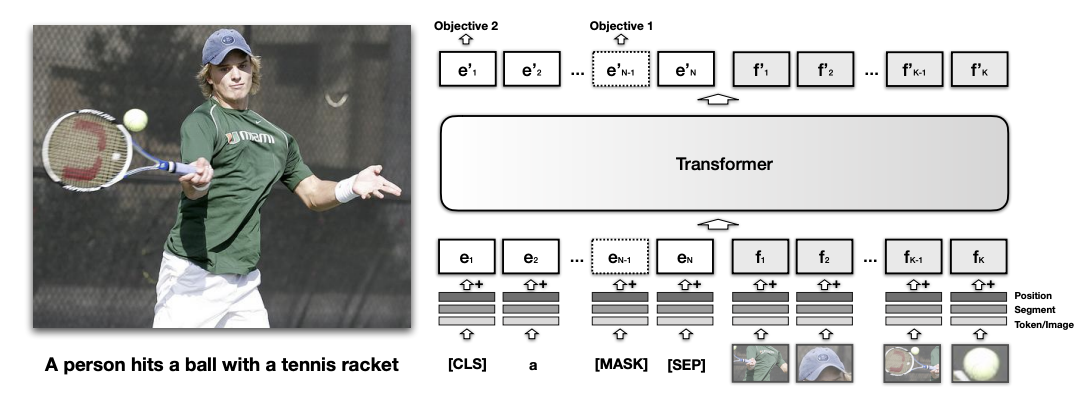
\includegraphics[width=0.8\linewidth]{./pic/ViBERT.png}}\\
    \subfloat[LXMERT \cite{tan2019lxmert}]{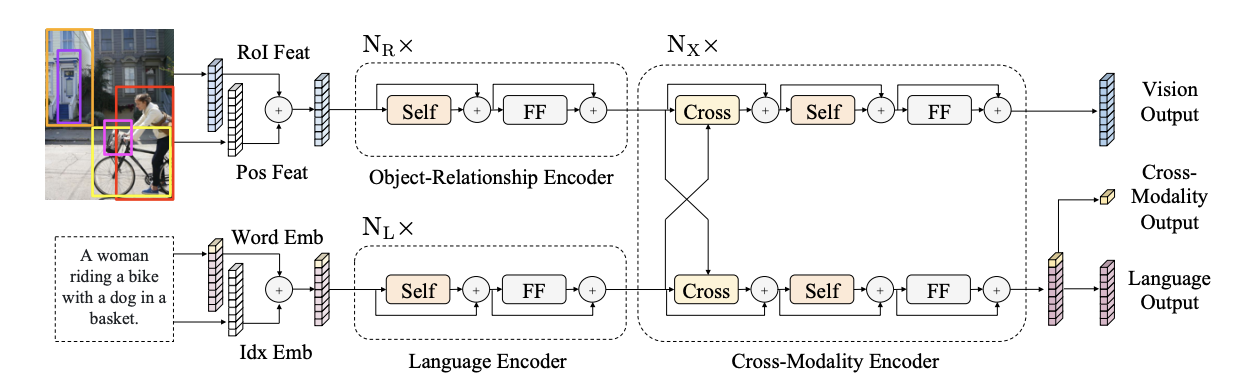
\includegraphics[width=0.8\linewidth]{./pic/LXMERT.png}}\\
    \subfloat[UNITER \cite{chen2020uniter}]{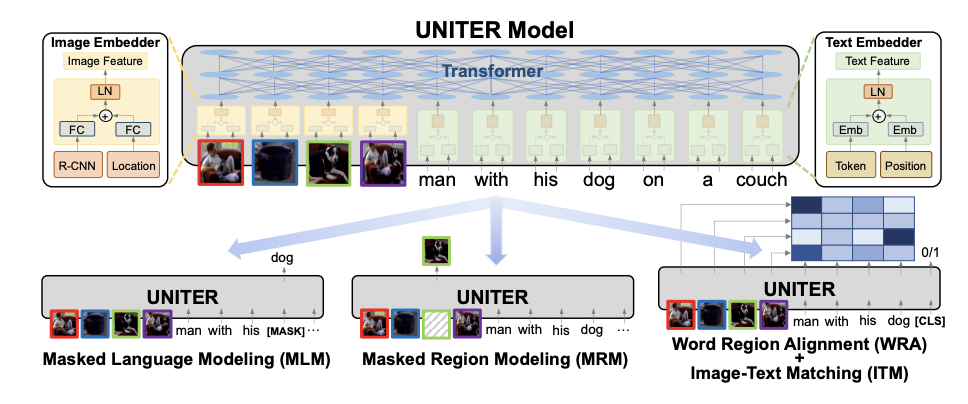
\includegraphics[width=0.8\linewidth]{./pic/UNITER.png}}
    \caption{Architectural of ViLBERT, LXMERT, and UNITER.}
    \label{fig:VLMs}
\end{figure}

Researchers have dedicated efforts to assess the ability of VLMs in comprehending commonsense spatial reasoning. Visual Question Answering (VQA) tasks have been employed to evaluate the performance of VLMs in answering questions that involve spatial relationships between objects depicted in images\cite{7410636}. Consequently, various benchmarks and question sets have been developed to specifically evaluate the spatial reasoning capabilities of VLMs.

For instance, Liu et al. (2022) meticulously curated an extensive dataset comprising more than 10,000 text-image pairs, encompassing a remarkable range of 66 distinct types of spatial relations \cite{liu2022visual}. Through their comprehensive evaluation, encompassing both human subjects and Virtual Language Models (VLMs), they illuminated the notable disparity between VLMs and human performance in this intricate task. Furthermore, to comprehensively assess the spatial reasoning capacities of VLMs, various benchmarks have been developed.

\begin{figure*}[tp]
    \centering
  \subfloat[a\label{1a}]{%
       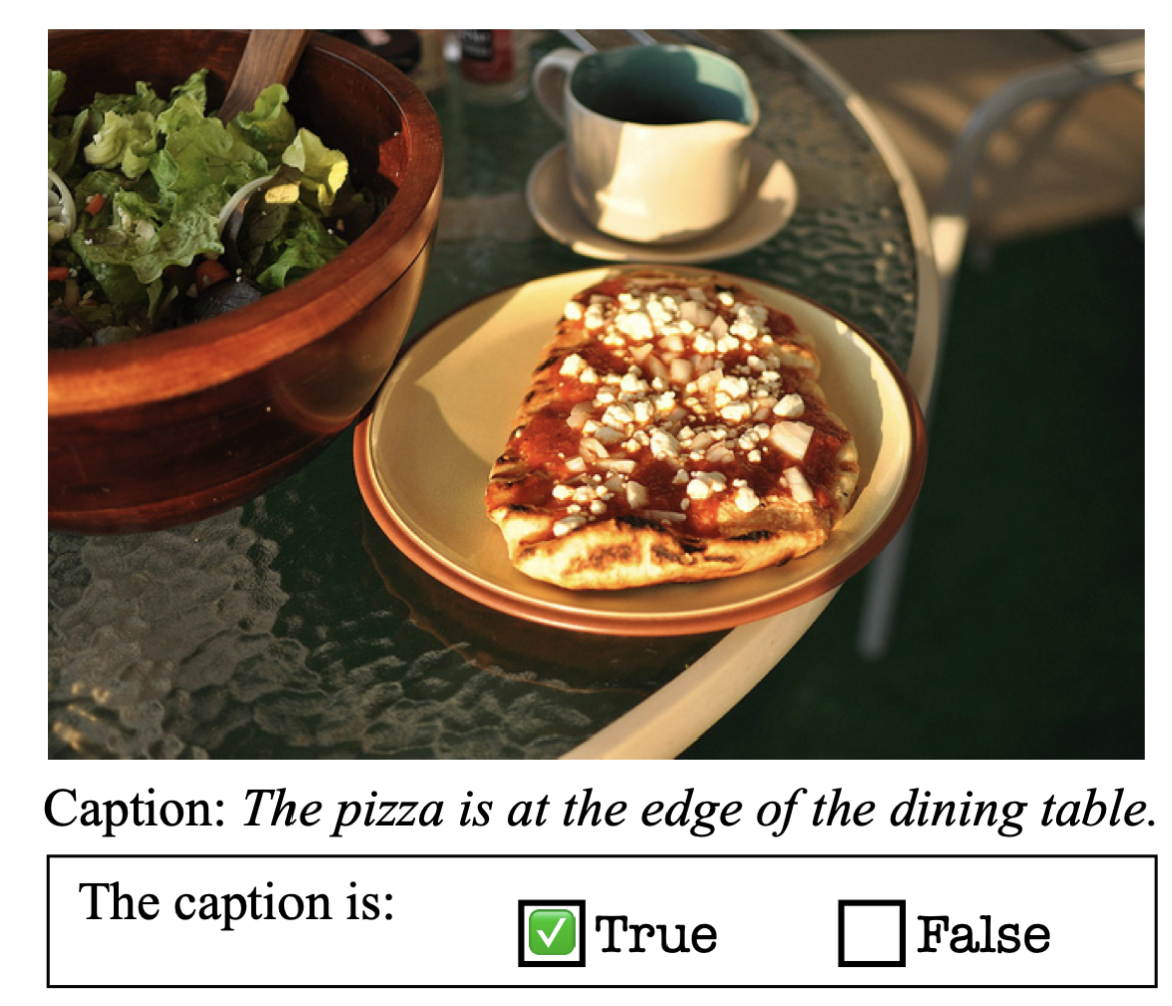
\includegraphics[width=0.45\linewidth]{./pic/Example of Bechmark.png}}
    \hfill
  \subfloat[b\label{1b}]{%
        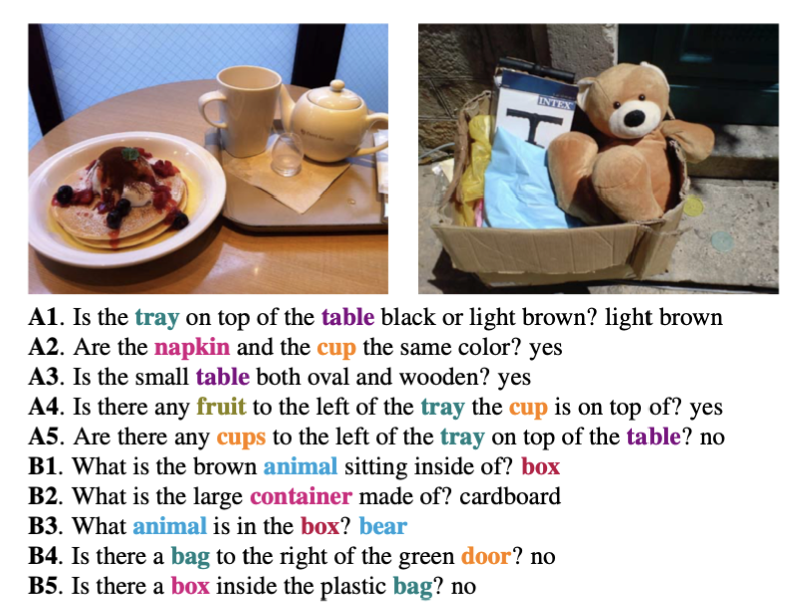
\includegraphics[width=0.45\linewidth]{./pic/GQA-example.png}}
    \\
  \subfloat[c\label{1c}]{%
        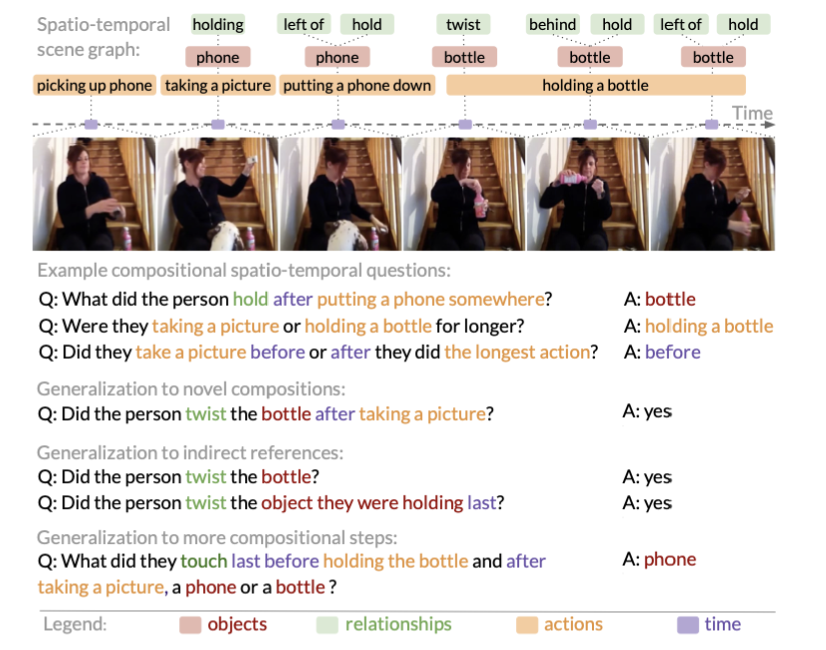
\includegraphics[width=0.45\linewidth]{./pic/AGQA-example.png}}
    \hfill
  \subfloat[d\label{1d}]{%
        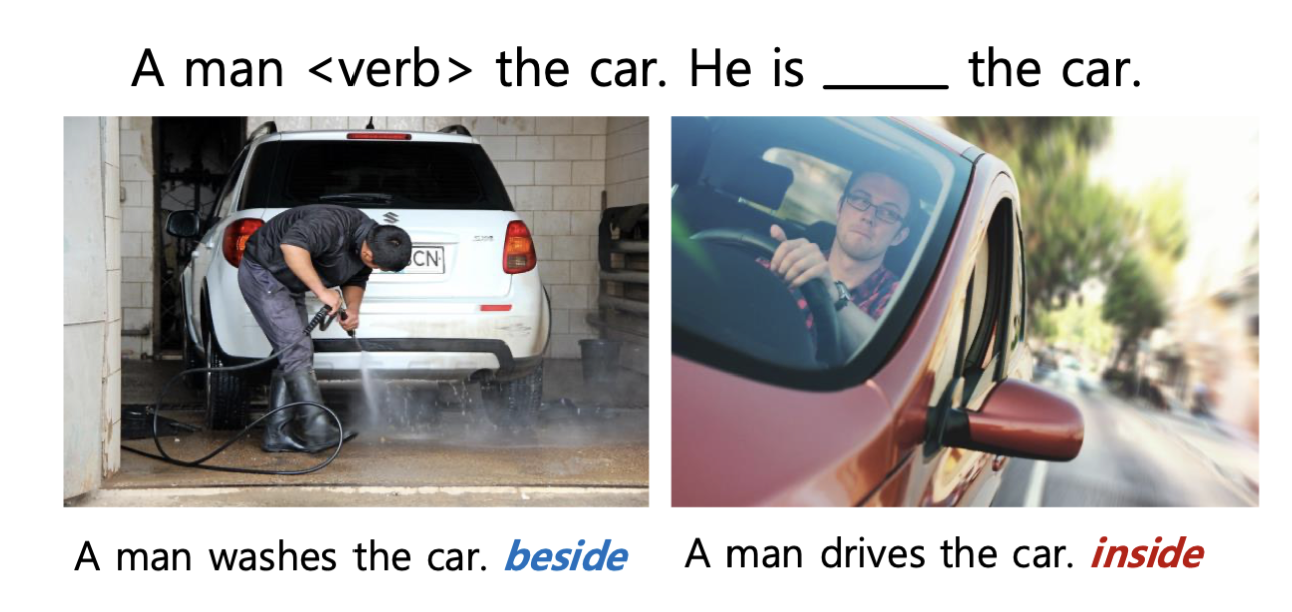
\includegraphics[width=0.45\linewidth]{./pic/example of B Liu.png }}
  \caption{Examples of spatial reasoning benchmarks. (a)Example in benchmark proposed by Liu et al. (2022) \cite{liu2022visual}  (b)Example questions and images of GQA \cite{hudson2019gqa}. (c)Example questions and images of AGQA \cite{grunde2021agqa}. (d)Example in benchmark proposed by Liu et al. (2021) it asks VLMs to give potential position between car and man. \cite{liu2022things}.}
  \label{fig:spatial_reasoning_benchmarks}
\end{figure*}

One such benchmark, GQA \cite{hudson2019gqa}, delves into the domain of question generation, pushing the boundaries of VLMs' ability to generate relevant questions. AGQA \cite{grunde2021agqa}, on the other hand, extends the evaluation to include video-based data, capturing the nuances of spatial reasoning in dynamic visual contexts. The Compositional Visual Relations Dataset \cite{zerroug2022benchmark} was meticulously constructed with a focus on Compositional Visual Relations (CVR), challenging VLMs with intricate visual relationships. VALSE \cite{parcalabescu2021valse} places its emphasis on unraveling the sensitivity of VLMs in spatial reasoning tasks, aiming to uncover their aptitude for subtle distinctions.

Furthermore, Liu et al. (2021) introduced a benchmark \cite{liu2022things} that scrutinizes the relative scales of objects, enabling a deeper exploration of VLMs' comprehension of spatial proportions. To capture a richer spectrum of spatial phenomena, SpartQA \cite{mirzaee2021spartqa} was meticulously devised, providing a challenging arena for evaluating VLMs' spatial reasoning capabilities.

Figure \ref{fig:spatial_reasoning_benchmarks} showcases a glimpse of these remarkable benchmarks, highlighting the efforts undertaken to assess and comprehend the spatial reasoning prowess of VLMs.


These benchmarks and datasets serve as valuable tools to assess the progress and limitations of VLMs in the realm of spatial reasoning and they have such things in common: (i) they are all based on commonsense spatial reasoning, (ii) they all focus on VLMs, (iii) they all only ask LLMs to use simple answers to these questions, like "yes" or "no", and (iv) they all given some bound words to the model to limit the model's answer space.

In conclusion, this literature review presents a thorough examination of the current landscape in the realm of LLMs and their Spatial Reasoning capabilities. It consolidates recent research from the fields of LLMs, Spatial Reasoning, and VQA, providing an in-depth analysis of the advancements made thus far. The review sheds light on the existing limitations and challenges that LLMs encounter when comprehending and reasoning about spatial relationships in visual content. Moreover, it offers valuable insights into potential strategies for enhancing LLMs' Spatial Reasoning abilities. By synthesizing these findings, this review contributes to a comprehensive understanding of the current state of the art in LLMs' Spatial Reasoning capabilities and paves the way for future advancements in this field.

\section{Development and Implementation Summary}
This project aims to investigate the Visual Spatial Reasoning capabilities of LLMs, specifically focusing on their performance in VQA tasks. So the development and implementation of this project will be divided into these parts:

\subsection{Probelm Identification}
The main problem of this project is to investigate the Spatial Reasoning abilities of LLMs, specifically focusing on their performance in VQA tasks. So the first step is to identify the problem and the research questions. The research questions are as follows:
\begin{enumerate}
    \item What are the Visual Spatial Reasoning abilities of LLMs?
    \item What are the limitations and challenges faced by LLMs in comprehending and reasoning about spatial relationships in visual content?
    \item What is the current state of Spatial Reasoning capabilities in leading LLMs?
    \item What are the potential avenues for enhancing LLMs' Spatial Reasoning abilities?
\end{enumerate}

\subsection{Experiment Design}
For the experimental stage, the workflow can be visualized as depicted in Figure \ref{fig:workflow}. The experiment is divided into three distinct parts, each serving a specific purpose:

\begin{figure}[htbp]
    \centering
    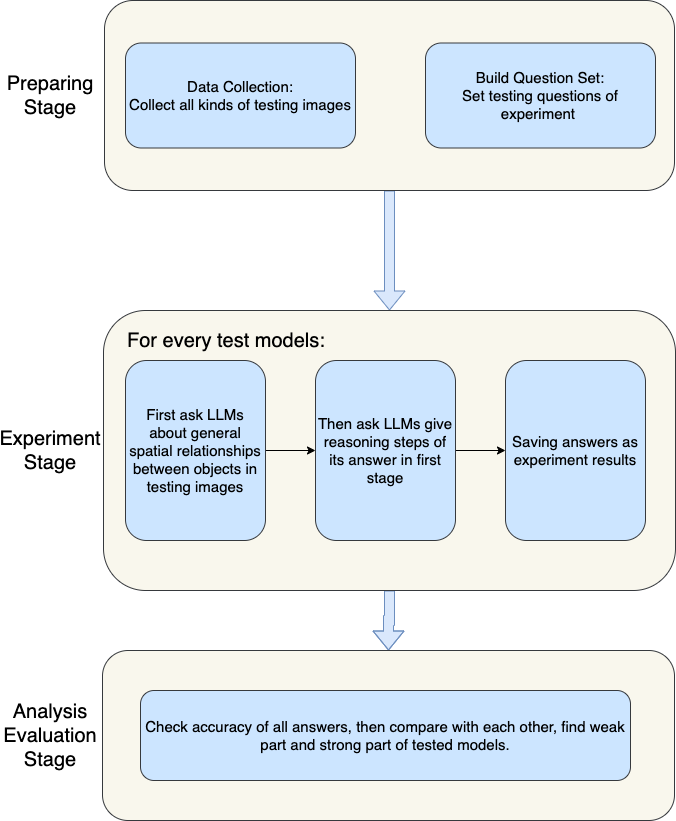
\includegraphics[width=0.8\linewidth]{./pic/workflow.drawio.png}
    \caption{Workflow of the experiment}
    \label{fig:workflow}
\end{figure}

\begin{enumerate}
    \item \textbf{Prepare Stage}
    \subitem During this stage, the primary objective is to gather a diverse collection of images that contain various spatial relations. These images can be sourced from the internet or generated using appropriate tools. For this project, the dataset will consist of a combination of an existing benchmark proposed by Liu et al. (2022) \cite{liu2022visual}.
    Another crucial aspect is the question set, which will be divided into three parts:
    \begin{itemize}
        \item Questions discussing the spatial relationships between objects depicted in the images.
        \item Questions requiring the reasoning steps behind the previous answers.
        \item Questions sets following the guidelines proposed by Burnell et al. (2023) and Davis(2023) \cite{burnell2023rethink,davis2023benchmarks}.
    \end{itemize}
    \item \textbf{Experiment Stage}
    \subitem The focus of this stage is to test different versions of Large Language Models (LLMs) using the prepared dataset and question set. The LLMs will be evaluated based on two factors:
    \begin{itemize}
        \item Different sizes of LLMs.
        \item Different pre-training methods of LLMs.
    \end{itemize}
    The experiment will involve running the LLMs on the prepared dataset, recording the results, and analyzing their performance. And all testing models will be GPT models, including from GPT-3.5 tubor to GPT-4-0612.
    \item \textbf{Analysis and Evaluation Stage}
    \subitem In this stage, the emphasis is on analyzing the performance of the different versions of LLMs using the prepared dataset. The analysis will primarily consider two aspects:
    \begin{itemize}
        \item The accuracy of the answers provided by the LLMs.
        \item The reasoning steps generated by the LLMs.
    \end{itemize}
    Based on the accuracy, the effectiveness and capability of the LLMs in spatial reasoning can be evaluated and compared. By examining the reasoning steps, any limitations and challenges faced by LLMs in comprehending and reasoning about spatial relationships in visual content can be identified.
\end{enumerate}

Through this systematic workflow, the experiment aims to assess the performance and capabilities of various versions of LLMs in spatial reasoning tasks. The analysis and evaluation stage provide insights into the strengths, weaknesses, and potential areas for improvement in LLMs' understanding and reasoning abilities pertaining to spatial relationships in visual content.

\subsection{Model Selection}
This project exclusively focuses on the utilization of GPT-series models due to their favorable characteristics and accessibility. Extensive research conducted on the Internet indicates that GPT-series models offer notable convenience compared to other models such as BERT, RoBERTa, and T5. The aforementioned models are deemed unsuitable for this project due to their limited support for text input exclusively. While models like ViBERT, ViT, and CLIP support both image and text inputs, they are not readily accessible on public websites. Although researchers have uploaded some training models on platforms like HuggingFace, their usage necessitates deployment on local machines, which requires high-performance experimental equipment that is not currently available for me. Conversely, GPT-series models are readily accessible on the OpenAI website and can be directly employed without the need for additional infrastructure, thus rendering them highly convenient for the purposes of this project.

\subsection{Question Template}
The question template is an important part of this project. The question template is shown as Table \ref{tab:question_template}. As shown in the table, the question template consists of two parts: the input image and the question. The input image is the image that will be used to test the LLMs. The question is the question that will be asked to the LLMs. The question template will be used to generate the question set.

\begin{table}[ht]
    \centering
    \caption{Question Template}
    \label{tab:question_template}
    \begin{tabular}{|p{0.4\linewidth}|p{0.5\linewidth}|}
        \hline
        \textbf{Input Image} &\textbf{Question}\\
        \hline
        \begin{center} 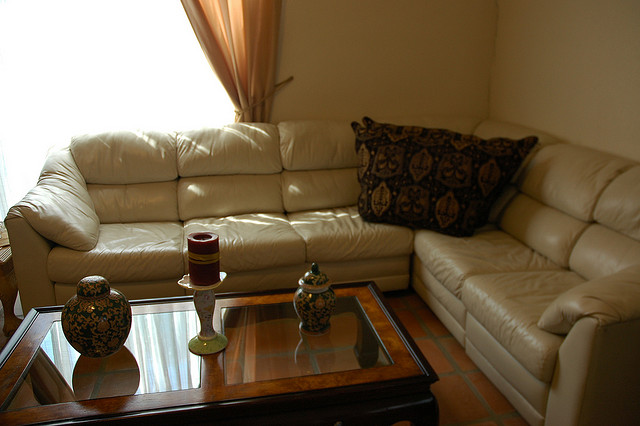
\includegraphics[width=\linewidth]{./pic/000000573553.jpg} \end{center}
        & \begin{enumerate}
            \item Can you describe the spatial relationship between the tea table and the sofa?
            \item Can you describe the relevant spatial relationships between the objects on the tea table?
            \item Show the Reasoning Steps.
        \end{enumerate}\\
        \hline
        \end{tabular}
\end{table}


\section{Data Sources}
The data utilized in this project will be divided into two main parts: the dataset and question set, and the answers generated by the Large Language Models (LLMs).

For the dataset and question set, a combination of existing benchmarks proposed by Liu et al. (2022) \cite{liu2022visual} and self-generated images will be used. The images in the dataset will encompass real-world objects along with 2D shapes, ensuring a diverse range of spatial relationships to be examined. The benchmark images are extracted from the COCO 2017 dataset \cite{lin2014microsoft}, which is an open-source dataset widely used in computer vision research. It is important to note that the usage of the COCO dataset has been granted full permission for this project.

As for the second part, the answers generated by the LLMs will be stored in a text file. The answers will be generated using the OpenAI website, which provides a platform for executing queries and obtaining responses from the language model. The generated answers can be conveniently downloaded as a text file from the website or saved directly on the platform.

By utilizing this comprehensive data setup, incorporating a combination of benchmark images and self-generated content, along with leveraging the power of LLMs to generate answers, the project aims to provide an extensive and diverse set of data for analysis and evaluation. The combination of the benchmark dataset and the generated answers will enable the project to assess the performance and capabilities of the LLMs in spatial reasoning tasks accurately.

It is important to ensure adherence to proper data usage policies, including obtaining necessary permissions for the benchmark dataset and complying with any licensing or attribution requirements associated with the dataset. This approach ensures the project's integrity and ethical practices while utilizing publicly available data resources for research purposes.

\section{Evaluation}
This project aims to assess the proficiency and capabilities of Large Language Models (LLMs) in comprehending and reasoning about spatial relationships within visual content. The evaluation will encompass two primary dimensions: the accuracy of LLM-generated answers and the quality of reasoning steps produced by LLMs. The evaluation will be conducted through the following methodologies:

\begin{enumerate}
    \item \textbf{Accuracy of Answers:} The accuracy of LLM-generated answers will be assessed by comparing them with the ground truth answers obtained through manual responses to the question set. The accuracy will be quantified by dividing the number of correct answers by the total number of questions.
    \item \textbf{Reasoning Steps:} The quality of reasoning steps generated by LLMs will be evaluated by comparing them to the ground truth reasoning steps, obtained through manual responses. The evaluation of reasoning steps will be based on the following criteria:
    \begin{itemize}
        \item \textbf{Correctness:} The generated reasoning steps should demonstrate accuracy and precision in their content.
        \item \textbf{Completeness:} The reasoning steps should provide comprehensive and exhaustive coverage of the underlying reasoning process.
        \item \textbf{Coherence:} The reasoning steps should exhibit logical coherence, ensuring a coherent flow of reasoning from initial premises to the final conclusions.
    \end{itemize}
\end{enumerate}

By employing these evaluation measures, this project seeks to gain insights into the effectiveness and soundness of LLMs in understanding and reasoning about spatial relationships.

\section{Ethical Considerations}
In the pursuit of investigating the Spatial Reasoning capabilities of LLMs within the context of VQA, it is essential to address several ethical considerations. These considerations ensure the responsible and ethical utilization of LLMs in the research and development process, while also mitigating potential risks and promoting equitable outcomes. The following ethical considerations should be given due attention:
\begin{enumerate}
    \item Bias and Fairness: LLMs rely on extensive amounts of training data, and if this data contains biases, the models may inadvertently perpetuate or amplify those biases. It is crucial to identify and address biases related to spatial relationships, objects, or cultural aspects within the training data. Fairness and inclusivity should be prioritized to avoid marginalization or discrimination based on protected characteristics such as race, gender, socioeconomic status, etc.
    \item Privacy and Confidentiality: Throughout the experiment, privacy rights and data protection regulations must be upheld. Careful attention should be given to the handling of any personally identifiable information (PII) and the implementation of appropriate anonymization techniques. Participants' privacy should be protected, and their data should be stored securely to prevent unauthorized access.
    \item Informed Consent: If human participants are involved in the data collection or evaluation process, obtaining informed consent is imperative. Participants should receive clear and comprehensive information about the purpose, procedures, and potential risks associated with their participation. They should have the freedom to make an informed decision about their involvement and the right to withdraw their consent at any point during the experiment.
    \item Transparency and Explainability: LLMs often operate as black boxes, making it challenging to understand how they arrive at their answers or reasoning steps. Efforts should be made to enhance the transparency and explainability of LLMs' decision-making processes in the context of Visual Spatial Reasoning. This includes providing clear explanations of the models' functioning and ensuring that the generated answers are interpretable and understandable.
    \item Responsible Research Practices: Throughout the experiment, researchers should adhere to rigorous scientific methodologies, ensuring the reliability and validity of the findings. This involves maintaining transparency in reporting the methodology, results, and limitations of the study. Rigorous peer review and open scientific discourse should be encouraged to foster accountability and rigor in the research community.
    \item Ethical AI Governance: As the capabilities of LLMs continue to advance, it is crucial to establish governance frameworks and accountability mechanisms specific to the development and deployment of these models in Spatial Reasoning applications. This may involve considering ethical guidelines, standards, and regulations that promote responsible and ethical practices, thereby safeguarding against potential risks and unintended consequences.
\end{enumerate}
By addressing these ethical considerations, researchers can ensure the responsible exploration of LLMs' Spatial Reasoning capabilities and contribute to the development of ethical guidelines in the field of Natural Language Processing (NLP). Moreover, these considerations uphold principles of fairness, transparency, and respect for individual rights, fostering a trustworthy and beneficial environment for both researchers and participants involved in such studies.

\section{Project Plan}
The project timeline and task allocation are visually represented in Figure \ref{fig:gantt}, showcasing the specific Gantt chart. The project is organized into four distinct stages, each comprising multiple tasks aimed at achieving the project objectives. The stages and their corresponding tasks are outlined below:

\begin{figure*}[hbp]
    \centering
    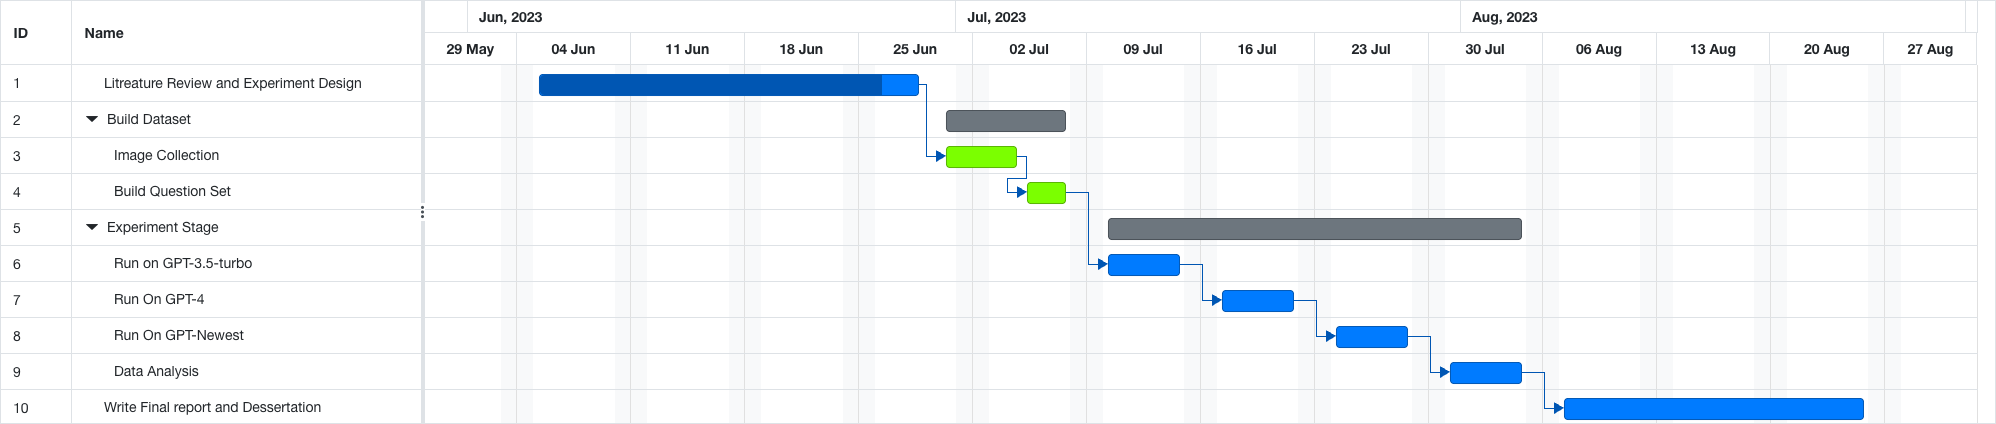
\includegraphics[width=0.8\linewidth]{./pic/Gnatt.png}
    \caption{Gantt Chart}
    \label{fig:gantt}
\end{figure*}

\begin{enumerate}
    \item Literature Review
    \subitem This stage focuses on conducting an extensive literature review to gain a comprehensive understanding of the project domain. It is divided into three tasks:
    \begin{itemize}
        \item Literature review: Conduct a thorough review of relevant research, technologies, and best practices in the field.
        \item Problem identification: Identify the key challenges and opportunities that the project aims to address.
        \item Experiment design: Plan and design the experimental framework and methodologies for subsequent stages.
    \end{itemize}
    \item Build Dataset
    \subitem In this stage, the focus is on creating the dataset and question set required for the experiments. It involves two tasks:
    \begin{itemize}
        \item Prepare dataset: Collect or curate a dataset comprising a combination of existing benchmark images and self-generated images.
        \item Prepare question set: Design and develop a set of questions that encompass various spatial relationships and reasoning scenarios.
    \end{itemize}
    \item Experiment Stage
    \subitem The experiment stage involves executing the designed experiments using the created dataset and question set. This stage is divided into two tasks:
    \begin{itemize}
        \item Run experiment: Implement the experiments using the selected Large Language Models (LLMs) and the prepared dataset and question set.
        \item Record results: Collect and document the results obtained from the experiments, ensuring comprehensive record-keeping.
    \end{itemize}
    \item Analysis and Evaluation Stage
    \subitem In this stage, the focus is on analyzing and evaluating the results obtained from the experiments. This stage comprises two tasks:
    \begin{itemize}
        \item Analyze results: Perform a detailed analysis of the experimental outcomes, considering the accuracy of answers and the reasoning steps generated by the LLMs.
        \item Evaluate results: Assess the performance and effectiveness of the LLMs in spatial reasoning, identify limitations, and recognize challenges faced by the models.
    \end{itemize}
    \item Final Report
    \subitem The final stage involves documenting the project outcomes in a report and preparing a presentation. It is divided into two tasks:
    \begin{itemize}
        \item Write report: Compile all the findings, methodologies, and conclusions into a comprehensive report that highlights the project's objectives, methodology, and results.
        \item Write presentation: Create a visually engaging presentation summarizing the project's key aspects, including objectives, methodology, results, and conclusions.
    \end{itemize}
\end{enumerate}

By following this well-structured project plan, the project aims to ensure efficient task allocation, timely execution, and a systematic approach towards achieving the project objectives. The defined stages and tasks provide a clear roadmap for project completion and successful delivery of the intended outcomes.

\section{Risks and Contingency Plans}
For this project, there are several risks that may affect the project progress. The risks and corresponding contingency plans are outlined in Table \ref{tab:risks} below:
\begin{table*}[ht]
    \centering
    \caption{Risks and Contingency Plans}
    \begin{tabular}{@{}cccc@{}}
    \toprule
    Risks            & Contingencies                                                      & Likelihood & Impact                     \\ \midrule
Website Break & To pervent this situation, I will limit the number questions in one time          & Medium & May delay the experiment progress  \\
Hardware Failure & I have backup hardware device to support me to continue experiment & Low        & Will casue project failure \\
Software Failure & If the software faliure, I can use API of opanai to continue works & Low        & Hardly influence project   \\
Dataset Issue & If the data source occur issues, I can use other sources to continue this project & Low    & Hardly influence project           \\
Model Update  & If there occur new version of models, I will add steps in experiment work         & Medium & Will delay the experiment progress \\ \bottomrule
    \end{tabular}
    \label{tab:risks}
\end{table*}


\bibliographystyle{IEEEtran}
\bibliography{mybib}

\end{document}